% Source: graduate-coursework/Sp26/CSCE763/Course_Assignments/HW1/HW1_CSCE_763_solutions.tex

\documentclass[border=4pt]{standalone}
\usepackage{amsmath}
\usepackage{amssymb}
\usepackage{graphicx}
\usepackage{tikz}
\usepackage{xcolor}
\usetikzlibrary{shapes.geometric, arrows.meta, positioning, patterns}

\definecolor{USC_Garnet}{HTML}{73000A}
\definecolor{USC_Sandstorm}{HTML}{FFF2E3}
\definecolor{USC_Black90}{HTML}{363636}
\definecolor{USC_Black70}{HTML}{5C5C5C}
\definecolor{USC_Black50}{HTML}{A2A2A2}
\definecolor{USC_Black10}{HTML}{ECECEC}
\definecolor{USC_Honeycomb}{HTML}{65780B}
\definecolor{USC_Atlantic}{HTML}{466A9F}
\definecolor{USC_Congaree}{HTML}{1F414D}
\definecolor{USC_Rose}{HTML}{CC2E40}
\definecolor{outputbg}{RGB}{245,245,245}

\begin{document}
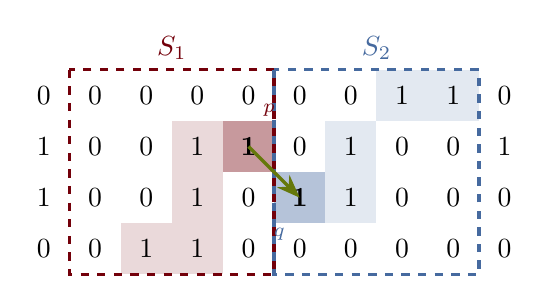
\begin{tikzpicture}[scale=0.65]
    % Background for V=1 pixels in S1
    \fill[USC_Garnet!15] (2.5,-0.5) rectangle (3.5,-1.5);
    \fill[USC_Garnet!15] (3.5,-0.5) rectangle (4.5,-1.5);
    \fill[USC_Garnet!15] (2.5,-1.5) rectangle (3.5,-2.5);
    \fill[USC_Garnet!15] (1.5,-2.5) rectangle (2.5,-3.5);
    \fill[USC_Garnet!15] (2.5,-2.5) rectangle (3.5,-3.5);
    % Background for V=1 pixels in S2
    \fill[USC_Atlantic!15] (6.5,0.5) rectangle (7.5,-0.5);
    \fill[USC_Atlantic!15] (7.5,0.5) rectangle (8.5,-0.5);
    \fill[USC_Atlantic!15] (5.5,-0.5) rectangle (6.5,-1.5);
    \fill[USC_Atlantic!15] (4.5,-1.5) rectangle (5.5,-2.5);
    \fill[USC_Atlantic!15] (5.5,-1.5) rectangle (6.5,-2.5);
    % Highlight the key pair
    \fill[USC_Garnet!40] (3.5,-0.5) rectangle (4.5,-1.5);
    \fill[USC_Atlantic!40] (4.5,-1.5) rectangle (5.5,-2.5);
    % Grid values
    \node at (0,0) {0}; \node at (1,0) {0}; \node at (2,0) {0}; \node at (3,0) {0}; \node at (4,0) {0};
    \node at (5,0) {0}; \node at (6,0) {0}; \node at (7,0) {1}; \node at (8,0) {1}; \node at (9,0) {0};
    \node at (0,-1) {1}; \node at (1,-1) {0}; \node at (2,-1) {0}; \node at (3,-1) {1}; \node[font=\bfseries] at (4,-1) {1};
    \node at (5,-1) {0}; \node at (6,-1) {1}; \node at (7,-1) {0}; \node at (8,-1) {0}; \node at (9,-1) {1};
    \node at (0,-2) {1}; \node at (1,-2) {0}; \node at (2,-2) {0}; \node at (3,-2) {1}; \node at (4,-2) {0};
    \node[font=\bfseries] at (5,-2) {1}; \node at (6,-2) {1}; \node at (7,-2) {0}; \node at (8,-2) {0}; \node at (9,-2) {0};
    \node at (0,-3) {0}; \node at (1,-3) {0}; \node at (2,-3) {1}; \node at (3,-3) {1}; \node at (4,-3) {0};
    \node at (5,-3) {0}; \node at (6,-3) {0}; \node at (7,-3) {0}; \node at (8,-3) {0}; \node at (9,-3) {0};
    % S1 / S2 boundaries
    \draw[dashed, very thick, USC_Garnet] (0.5,0.5) rectangle (4.5,-3.5);
    \node[above, USC_Garnet, font=\bfseries] at (2.5,0.5) {$S_1$};
    \draw[dashed, very thick, USC_Atlantic] (4.5,0.5) rectangle (8.5,-3.5);
    \node[above, USC_Atlantic, font=\bfseries] at (6.5,0.5) {$S_2$};
    % Arrow between key pair
    \draw[-{Stealth}, very thick, USC_Honeycomb] (4,-1) -- (5,-2);
    % Labels
    \node[above right, USC_Garnet, font=\scriptsize\bfseries] at (4.1,-0.6) {$p$};
    \node[below left, USC_Atlantic, font=\scriptsize\bfseries] at (4.9,-2.4) {$q$};
\end{tikzpicture}
\end{document}
